\textbf{Ejemplo 10}\\
¿Cuánto debe crecer linealmente una serie de 8 egresos efectuados al final de cada período y cuyo primer egreso es de 600{.}000COP para que, puesta en valor presente, sea equivalente a una serie de 10 egresos que crecen geométricamente en un 25\% y cuyo primer egreso es de  100.000 COP? Suponga una tasa del 3\% periódica anual vencida.\\

	%%%%%%%%%%%%%%%%%%% EJERCICIO 10 %%%%%%

%\newpage %USAR SOLO SI EL SOLUCIÓN QUEDA SOLO Y ES NECESARIO BAJARLO A LA SIGUIENTE PAGINA
\textbf{Solución.}\\
%La tabla ira centrada
\begin{center}
	\renewcommand{\arraystretch}{1.6}% Margenes de las celdas
	%Creación de la cuadricula de 3 columnas
	\begin{longtable}[H]{|c|c|c|}
		%Creamos una linea horizontal
		\hline
		%Definimos el color de la primera fila
		\rowcolor[HTML]{FFB183}
		%%%%% INICIO ASIGNACIÓN FECHA FOCAL %%%%%%%
		%%%%%%%%%% INICIO TITULO
		%Lo que se hace aquí es mezclar las 3 columnas en una sola
		\multicolumn{3}{|c|}{\cellcolor[HTML]{FFB183}\textbf{1. Asignación período focal}}  \\ \hline
		\multicolumn{3}{|c|}{$pf = \textit{0 pav}$}   \\\hline
		%%%%%%%%%% FIN TITULO
		%%%%% INICIO DECLARACIÓN DE VARIABLES %%%%%%%
		%%%%%%%%%% INICIO TITULO
		%Lo que se hace aquí es mezclar las 3 columnas en una sola
		\multicolumn{3}{|c|}{\cellcolor[HTML]{FFB183}\textbf{2. Declaración de variables}}   \\ \hline
		%%%%%%%%%% FIN TITULO
		%%%%%%%%%% INICIO DE MATEMÁTICAS
		%Cada & hace referencia al paso de la siguiente columna
		
		\multicolumn{2}{|c|}{$\hspace{2 cm}R_1=  600{.}COP \hspace{2 cm}$} & $g=25\% \textit{crecimiento geométrico periódico con } g \neq i$ \\
		\multicolumn{2}{|c|}{$\hspace{2 cm}R_2= 100{.}000 COP \hspace{2 cm}$} & $n_1=8 \textit{ pav}$ \\
		\multicolumn{2}{|c|}{$\hspace{2 cm}i=3\% \textit{ pav} \hspace{2 cm}$} & $n_2=3\textit{ pav}$ \\
		\multicolumn{2}{|c|}{$\hspace{2 cm}L= ?COP   \hspace{2 cm}$} & \\ \hline	
		
		
		%%%%%%%%%% FIN DE MATEMÁTICAS
		%%%%% FIN DECLARACIÓN DE VARIABLES
		
		%%%%% INICIO FLUJO DE CAJA
		\rowcolor[HTML]{FFB183}
		\multicolumn{3}{|c|}{\cellcolor[HTML]{FFB183}\textbf{3. Diagrama de flujo de caja}} \\ \hline
		%Mezclamos 3 columnas y pondremos el dibujo
		%%%%%%%%%%%%% INSERCIÓN DE LA IMAGEN
		%Deberán descargar las imágenes respectivas del drive y pegarlas en la carpeta
		%n_capitulo/img/ejemplos/1/capitulo1ejemplo1.pdf  (el /1/ es el numero del ejemplo)
		\multicolumn{3}{|c|}{\textbf{Deuda inicial}} \\ 
		\multicolumn{3}{|c|}{ 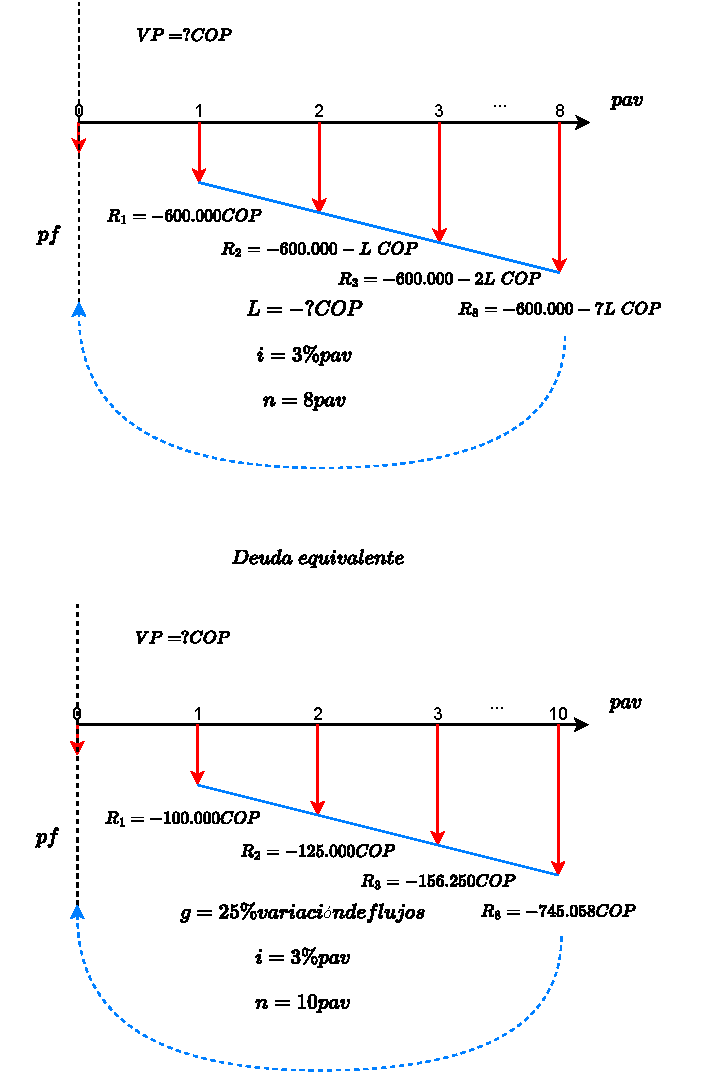
\includegraphics[trim=-5 -5 -5 -5 , scale=0.8]{6_Capitulo/img/ejemplos/10/Capitulo6Ejemplo10.pdf} } \\ \hline
		%%%%%%%%%%%%% FIN INSERCIÓN DE IMAGEN
		%%%%%FIN FLUJO DE CAJA
		
		%%%%% INICIO DECLARACIÓN FORMULAS
		%%%%%%%%%%% INICIO TITULO
		\rowcolor[HTML]{FFB183}
		\multicolumn{3}{|c|}{\cellcolor[HTML]{FFB183}\textbf{4. Declaración de fórmulas}}    \\ \hline
		%%%%%%%%%%% FIN TITULO
		%%%%%%%%%%% INICIO MATEMÁTICAS
		
		\multicolumn{3}{|c|}{$VP=\frac{(R)(1+i)^{n}-1}{i(1+i)^{n}}+\frac{L}{i}[\frac{(1+i)^{n}-1}{i(1+i)^{n}}-n(1+i)^{-n}] \hspace{0.4 cm} \textit{Valor presente de un gradiente aritmetico}$} \\
		\multicolumn{3}{|c|}{$VP=(\frac{(R)[(1+g)^{n}(1+i)^{-n}]-1}{g-i}) \hspace{0.4 cm} \textit{Valor presente de un gradiente geometrico si } g \neq i$} \\ \hline
		
		%%%%%%%%%% FIN MATEMÁTICAS
		%%%%%% INICIO DESARROLLO MATEMÁTICO
		\rowcolor[HTML]{FFB183}
		%%%%%%%%%%INICIO TITULO
		\multicolumn{3}{|c|}{\cellcolor[HTML]{FFB183}\textbf{5. Desarrollo matemático}}       \\ \hline
		%%%%%%%%%% FIN TITULO
		%%%%%%%%%% INICIO MATEMÁTICAS
		\multicolumn{3}{|c|}{\textit{Debemos igualar el valor de las dos series y despejar L: }} \\
		\multicolumn{3}{|c|}{$VP=\frac{(  600{.}000COP)[(1+0.03)^{8}-1]}{0.03(1+0.03)^{8}}+\frac{L}{0.03}[\frac{(1+0.03)^{8}-1}{0.03(1+0.03)^{8}}-8(1+0.03)^{-8}] $} \\
		\multicolumn{3}{|c|}{$VP=(\frac{(  100{.}000COP)[(1+0.25)^{10}(1+0.03)^{-10}-1]}{0.25-0.03}) $} \\ 
		\multicolumn{3}{|c|}{$VP= 2{.}695{.}415 COP$} \\ 
		\multicolumn{3}{|c|}{$2{.}695{.}415COP= 4{.}211{.}815COP+\frac{L}{0.03}*0.7044$} \\
		\multicolumn{3}{|c|}{$L= -64{.}582 COP$} \\ \hline
		%%%%%%%%%% FIN MATEMÁTICAS
		%%%%%% FIN DESARROLLO MATEMÁTICO
		%%%%%% INICIO RESPUESTA
		\rowcolor[HTML]{FFB183}
		%%%%%%%%%%INICIO TITULO
		\multicolumn{3}{|c|}{\cellcolor[HTML]{FFB183}\textbf{6. Respuesta}}   \\ \hline
		%%%%%%%%%% FIN TITULO
		%%%%%%%%%% INICIO RESPUESTA MATEMÁTICA
		\multicolumn{3}{|c|}{${L= -64{.}582 COP}$} \\ \hline
		%%%%%%%%%% FIN MATEMÁTICAS
		%%%%%% FIN RESPUESTA
	\end{longtable}
	%Se crean dos lineas en blanco para que no quede el siguiente texto tan pegado
	%\newline \newline %USARLO SI CREES QUE ES NECESARIO
\end{center}
%%%%%%%%%%%%%%%%%%%%%%%%%%FIN EJERCICIO 10 %%%%%%%%%%%%%%%%%%%%%%%%%%%
